\documentclass[titlepage]{article}
\usepackage{graphicx, float, tabularx, makecell, booktabs, amssymb}
\usepackage[a4paper, total={6in, 8in}]{geometry}
\usepackage[numbers]{natbib}
\usepackage{gensymb}
\setlength{\parskip}{1ex}

\title{\textbf{Are Clouds Fractal?}}
\author{Ansel Ong Ming Jin}
\date{\parbox{\linewidth}{\centering%
  July 2024 \endgraf\bigskip
  \textbf{Supervisor Team:} Dr Adam Povey, Dr Kamil Mroz\endgraf\medskip
  SURE2024 Scheme \endgraf\medskip
  University of Leicester}}

\begin{document}

\maketitle

\section{Introduction}

Clouds play an important role in the climate of regulating energy in the atmosphere as they can reflect energy from the Sun back into space and trap energy emitted from the Earth’s surface. This effect is quite significant considering that clouds cover about 70\% of the Earth’s surface at any given time. Many previous studies have calculated the fractal dimension of clouds when seen from a top down view using a geostationary satellite. The goal of this project is to determine whether clouds are also fractal based on the vertical cross sections of clouds acquired from ground-based remote sensing data. Section 2 shows a summary of the background research taken before starting the project. Section 3 will describe the datasets and approach used in this project. Section 4 discusses the results achieved and potential ideas for future work.

\section{Literature Survey}

\begin{table}[H]
    \begin{tabularx}{\textwidth}{*{6}{X}}
        \toprule
        Author(s) & Purpose & Fractal Dimension & Cloud Area & Image Source & Spatial Resolution\\
        \toprule
        Lovejoy (1982) & To determine if rain and cloud perimeters are fractals & 1.35 & \(1-1.2\times10^6\ km ^2\) & GOES & 4.8 km\\
        \hline
        Gotoh and Fujii (1998) & To propose a technique for cloud segmentation over land & \makecell[lt]{1.36\\1.68} & \makecell[lt]{\(<0.7\ km^2\)\\\(>0.7\ km^2\)} & Landsat TM & 30 m\\
        \hline
        Batista-Tomás et al. (2015) & To demonstrate that cirrus and cumulonimbus can be differentiated by their fractal dimension & 1.37 (cirrus)\newline1.18 (cumulonimbus) & \(>200 \ km^2\) & GOES 13 & 1 km\\
        \hline
        Christensen and Driver (2021) & To determine if global storm-resolving models can reproduce the fractal nature of clouds & \makecell[lt]{1.40\\1.50\\1.34\\1.39} & \(\geqslant 24\ px\) & \makecell[lt]{Himawari 8\\ICON\\IFS\\NICAM} & \makecell[lt]{5 km\\2.5 km \\4.8 km\\3.5 km}\\
        \bottomrule
    \end{tabularx}
    \caption{Previous papers that have calculated the fractal dimensions of clouds \cite{lovejoy1982area, gotoh1998fractal, batista2016classification, christensen2021fractal}}
    \label{tab:my_label}
\end{table}

\section{Methodology}

\subsection{Data}

Images of the vertical cross section of clouds were taken from the Aerosols, Clouds and Trace Gases Research Infrastructure (ACTRIS) Cloudnet data portal. Cloud data across 4 sites, namely Chilbolton, Galați, Munich, and Lindenberg, spanning the dates from 1 May 1999 to 31 March 2024 were used \cite{constantin2024, grsdorf2024}. Certain dates did not contain data for some or all sites. The data downloaded from the online portal was in the format of NetCDF files, which was converted to PNG files using the CloudnetPy Python Package \cite{Tukiainen2020}. The ECMWF Reanalysis v5 (ERA5) dataset was used to determine wind speeds and directions for each cloud at a range of altitudes and over time periods.

\subsection{Cloud Area Extraction}

\begin{figure}[h]
    \centering
    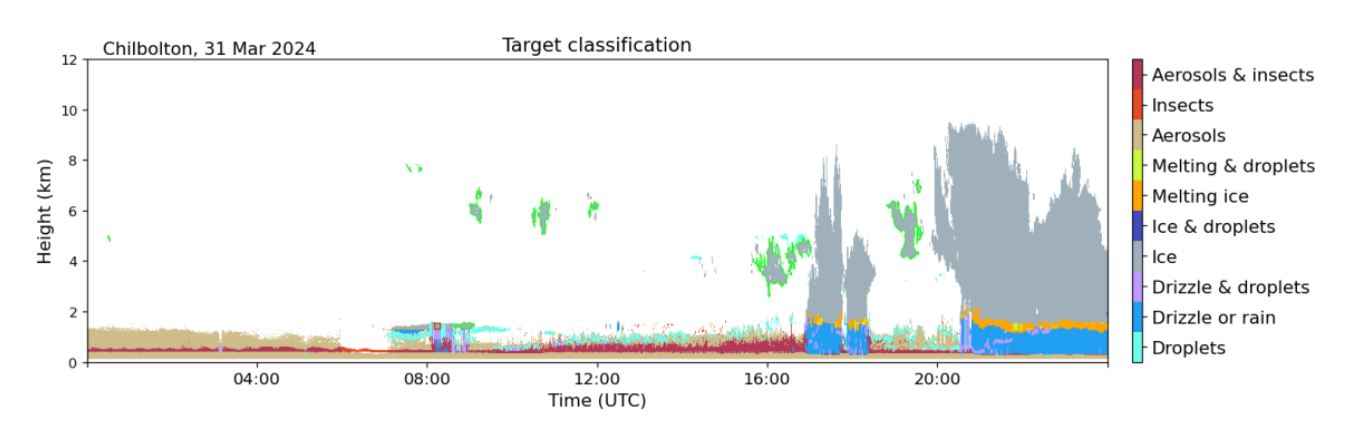
\includegraphics[width=0.75\linewidth]{fig1.png}
    \caption{Example image containing the vertical cross section of clouds from ACTRIS with clouds extracted highlighted using a green border}
    \label{fig:enter-label}
\end{figure}

Figure 1 shows an example of the images used to extract clouds. Ice clouds were extracted using colour detection to find contours around them. Liquid clouds were not used as their size is often underestimated due to weaker lidar signal penetration. As these images are showing the clouds that pass over a 24-hour period, clouds that span across days, meaning part of it is cut off, are filtered out as the full perimeter cannot be extracted. Clouds with a pixel area of less than 24 are also filtered out as the resolution is not high enough to calculate an accurate fractal dimension \cite{christensen2021fractal}. Clouds that are precipitating (connected to melting ice) are also filtered out as the shape of the bottom is flattened.

\subsection{Fractal Dimension Calculation}

The area-perimeter relation is used to calculate the fractal dimension of clouds. The relation can be written as the following equation:

\[P=k\cdot A^{D/2}\]
where P = perimeter, A = area, D = fractal dimension, and k is a constant.

After finding the contours of the clouds, it is easy to find the area and perimeter in pixels. However, using the size of the clouds in kilometres would give a more realistic result. The y-axis of the graph is already in kilometres, but the x-axis would need to be converted into kilometres to scale the value of area and perimeter in pixels into kilometres. The wind speeds of the clouds are needed to convert time into distance, giving the length of the cloud. The ERA5 dataset contains wind speeds at every model level, every hour, every latitude and longitude at intervals of 0.25\degree. To get the model level that the clouds reside on, the geopotential height of each model level needs to be calculated using the surface pressure, temperature, and specific humidity also provided by the dataset. Big clouds may have different wind speeds at different regions, e.g. the top area of the cloud usually has a higher wind speed than the lower area. For this project, all the wind speeds are averaged for simplification.

\section{Results and Conclusions}

\begin{figure}[h]
    \centering
    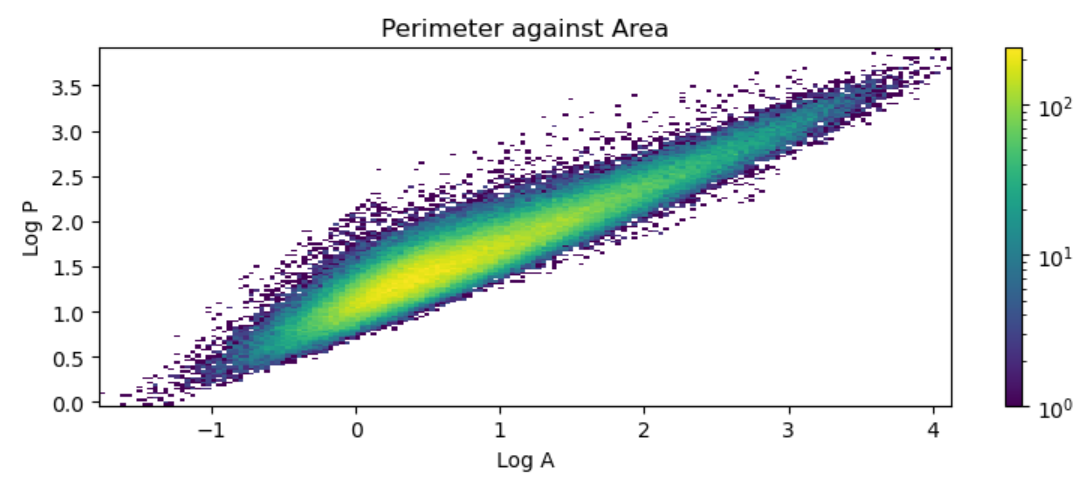
\includegraphics[width=0.75\linewidth]{fig2.png}
    \caption{Graph of Log of Perimeter against Log of Area}
    \label{fig:enter-label}
\end{figure}

Figure 2 shows the results of plotting all cloud areas and perimeters. The fractal dimension of the clouds can be calculated by multiplying the slope of the line by two, giving a value of \(D_{fractal}=1.26\). The linear nature of the plot shows that the vertical cross section of clouds also exhibit fractal behaviour. There are some improvements that could potentially increase the accuracy of the fractal dimension calculated. Many of the clouds extracted were actually clumps of smaller clouds that were categorised as one due to their pixels being in contact. Watershed segmentation was attempted in this paper with little success in dividing large clumps of clouds naturally. Different segmentation techniques such as instance segmentation could display a better performance. Another potential idea for future work is to take the different wind speeds and scale different regions of clouds accordingly.

\bibliographystyle{IEEEtranN}
\bibliography{references}

\end{document}
